\documentclass[11pt]{article}
\usepackage[fleqn]{amsmath}\textwidth 6.5in
\oddsidemargin -0.25in
%\evensidemargin -0.5in
\topmargin -0.25in
\textheight 9.2in

\newcommand{\docname}{\bf wvs-048}
\newcommand{\docdate}{22 October 2006}

\usepackage{graphicx}

\usepackage{floatflt}

\begin{document}

%\tracingcommands=1
\newlength{\hW} % heading box width
\newlength{\pW} % page number field width
\settowidth{\hW}{\docname}
\settowidth{\pW}{Page \pageref{lastpage}\ of \pageref{lastpage}}
\ifdim \pW > \hW \setlength{\hW}{\pW} \fi
\makeatletter
\def\@biblabel#1{#1.}
\newcommand{\ps@twolines}{%
  \renewcommand{\@oddhead}{%
    \docdate\hfill\parbox[t]{\hW}{{\hfill\docname}\newline
                          Page \thepage\ of \pageref{lastpage}}}%
\renewcommand{\@evenhead}{}%
\renewcommand{\@oddfoot}{}%
\renewcommand{\@evenfoot}{}%
}%
\makeatother
\pagestyle{twolines}

\vspace{-10pt}
\begin{tabbing}
\phantom{References: }\= \\
To: \>Bill\\
Subject: \>Different solution for $\phi$--$H$ calculation in {\tt metrics\_m}\\
From: \>Van Snyder\\
\end{tabbing}

\parindent 0pt \parskip 10pt
\vspace{-20pt}

\begin{floatingfigure}{3.75in}
{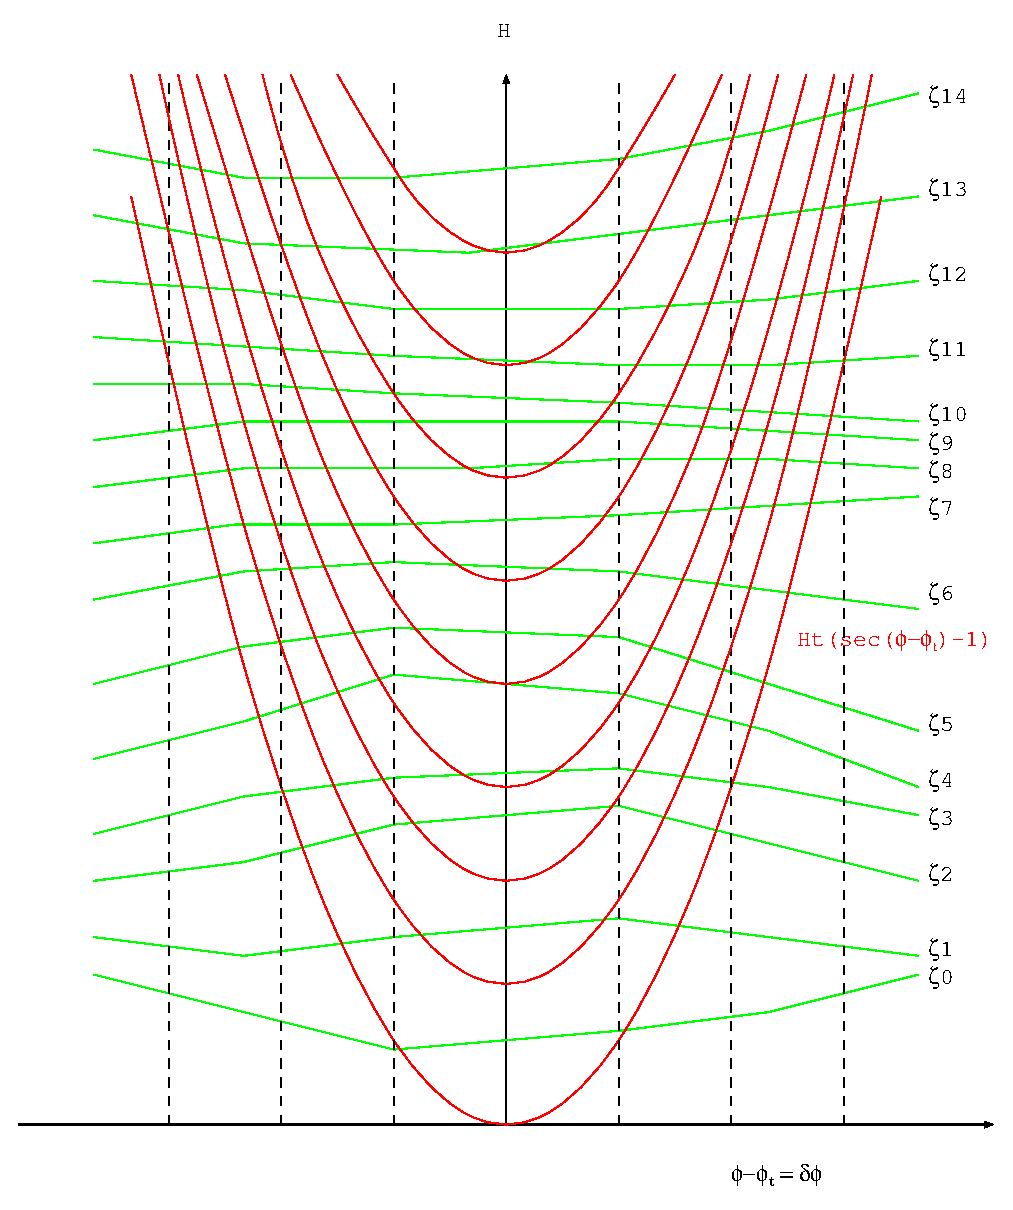
\includegraphics[width=3.5in,height=4.5in,clip]{./wvs-048-grid2.eps}}
\end{floatingfigure}

I drew the picture of the line of sight intersecting the $\zeta$ surfaces
in cartesian $\phi$--$H$ co\"{o}rdinates instead of polar  $\phi$--$\zeta$
co\"{o}rdinates.  In this diagram, the con\-stant-$\zeta$ surfaces are the
green lines, the line of sight is the red line, and the temperature $\phi$
basis is the vertical black lines.  Therefore the values of $H$ in the
{\tt H\_ref} array appear at the intersections of the green lines and the
vertical black lines.

Assuming the constant-$\zeta$ surfaces to be piecewise linear, this
suggests a simple algorithm to solve for the $\phi$ coordinate of each
intersection of the red line (the line of sight) with the green lines (the
constant-$\zeta$ surfaces).

Denote {\tt H\_ref} by $H$.  Between two consecutive columns of a row of
$H$ there is a line segment of a constant-$\zeta$ surface.  Writing the
intersection of that line with the line of sight expressed as a function
of $\phi$, \emph{viz.} $H-H_t = H_t(\sec \phi - 1)$, we need to solve

\begin{equation*}
H_{ij} + (H_{i,j+1}-H_{ij})
                  \frac{\phi-\phi_j}
                       {\phi_{j+1}-\phi_j} - H_t
= H_t(\sec \phi - 1)
\end{equation*}

or, using $\sec\phi \approx 1 + \frac12 \phi^2$ and putting the resulting
polynomial in standard form,

\begin{equation*}
\frac12 (\phi_{j+1}-\phi_j) H_t \phi^2 -
(H_{i,j+1}-H_{ij})\phi -
H_{ij} \phi_{j+1} + H_{i,j+1} \phi_j +
(\phi_{j+1}-\phi_j)H_t
\approx 0
\end{equation*}

for all $i$ and $j$, discarding solutions for which $\phi<\phi_j$ or
$\phi>\phi_{j+1}$.  The next term in the expansion of $\sec\phi$ is
$\frac5{24}\phi^4$ for $\phi$ in radians, or
$\frac5{24}\left(\frac{\pi}{180}\right)^4\phi^4 \approx
9.3\times10^{-8}\phi^4$ for $\phi$ in degrees, so this simple quadratic
equation is probably accurate enough.  Since this isn't an iterative
solution, do we still need to add the minimum $\zeta$ to the grid?

\label{lastpage}
\end{document}
% $Id$
